\documentclass[tikz,border=2pt]{standalone}
\usepackage{amsmath,amssymb}
\usepackage{tikz}
\usetikzlibrary{matrix}

\begin{document}
% Splitting the variables into x (p of them) and y (q of them) splits the Jacobian of
% F: R^{p+q} -> R^m into two blocks of columns, D_x F and D_y F.
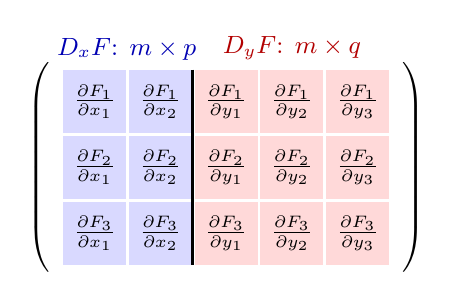
\begin{tikzpicture}[every node/.style={font=\small}]
	\matrix (J) [matrix of math nodes, nodes={minimum size=8mm, anchor=center}, left delimiter=(, right delimiter=), column sep=1pt, row sep=1pt] at (0,0) {
		|[fill=blue!15]| \tfrac{\partial F_1}{\partial x_1} & |[fill=blue!15]| \tfrac{\partial F_1}{\partial x_2} & |[fill=red!15]| \tfrac{\partial F_1}{\partial y_1} & |[fill=red!15]| \tfrac{\partial F_1}{\partial y_2} & |[fill=red!15]| \tfrac{\partial F_1}{\partial y_3} \\
		|[fill=blue!15]| \tfrac{\partial F_2}{\partial x_1} & |[fill=blue!15]| \tfrac{\partial F_2}{\partial x_2} & |[fill=red!15]| \tfrac{\partial F_2}{\partial y_1} & |[fill=red!15]| \tfrac{\partial F_2}{\partial y_2} & |[fill=red!15]| \tfrac{\partial F_2}{\partial y_3} \\
		|[fill=blue!15]| \tfrac{\partial F_3}{\partial x_1} & |[fill=blue!15]| \tfrac{\partial F_3}{\partial x_2} & |[fill=red!15]| \tfrac{\partial F_3}{\partial y_1} & |[fill=red!15]| \tfrac{\partial F_3}{\partial y_2} & |[fill=red!15]| \tfrac{\partial F_3}{\partial y_3} \\
	};
	\draw[thick] (J-1-2.north east) -- (J-3-2.south east);
	\node[blue!70!black, anchor=south] at (J-1-1.north east) {$D_xF$: $m\times p$};
	\node[red!70!black, anchor=south] at (J-1-4.north) {$D_yF$: $m\times q$};
\end{tikzpicture}
\end{document}
